\subsection{Stabilité}
\label{subsec:stabilite}

\subsubsection{Méthodologie}
\label{subsubsec:stabilite_methode}

L'analyse de la stabilité de la fusée SP-02 a été réalisée en utilisant deux outils principaux : \gls{Stabtraj} et \gls{OpenRocket}. Ces
logiciels permettent de modéliser la fusée, d'analyser ses caractéristiques aérodynamiques et de simuler son comportement en vol. La
méthodologie suivie pour l'analyse de la stabilité comprend les étapes suivantes:\\

\begin{enumerate}
    \item \textbf{Modélisation \acrshort{CAO} :} La fusée SP-02 a été modélisée en détail dans un logiciel de \acrshort{CAO}, en tenant
    compte des dimensions, de la géométrie et de la répartition des masses de chaque composant.\\
    
    \item \textbf{Importation dans \gls{OpenRocket} :} Après avoir finalisé la modélisation \acrshort{CAO}, le modèle a été construit dans
    le logiciel \gls{OpenRocket} à partir de ces brics de construction. Cette étape permet essentiellement de placer les différents éléments
    de la fusée et de leur attribuer des matériaux. Cela permet de définir la masse et le \acrfull{CdG} de chaques éléments et donc de
    la fusée dans son ensemble. Aussi, \gls{OpenRocket} permet d'estimer les caractéristiques aérodynamiques de la fusée, telles que le
    coefficient de traînée ($C_d$), le coefficient de portance ($C_l$) et le \acrfull{CdP}, en fonction de la géométrie et des conditions
    de vol.\\

    \item \textbf{Importation dans \gls{Stabtraj} :} Le modèle de la fusée a ensuite été importé dans \gls{Stabtraj} en comptant la masse et
    le \acrshort{CdG} ainsi que le $C_d$ fournis par \gls{OpenRocket}. En utilisant ces données, \gls{Stabtraj} permet de calculer le
    \acrshort{CdP} à partir de l'approximation de Barrowman \cite{Stab_doc} et d'analyser la stabilité longitudinale de la fusée.\\

    \item \textbf{Correction et itérations :} Si les résultats de l'analyse de stabilité indiquent que la fusée n'est pas stable, des
    ajustements sont effectués sur la conception, tels que le déplacement du \acrshort{CdG} ou la modification de la géométrie des surfaces
    de portances. La nouvelle conception est ensuite réévaluée en répétant les étapes précédentes jusqu'à obtenir une stabilité
    satisfaisante.\\
\end{enumerate}

\vfill

\begin{figure}[h!]
    \centering
    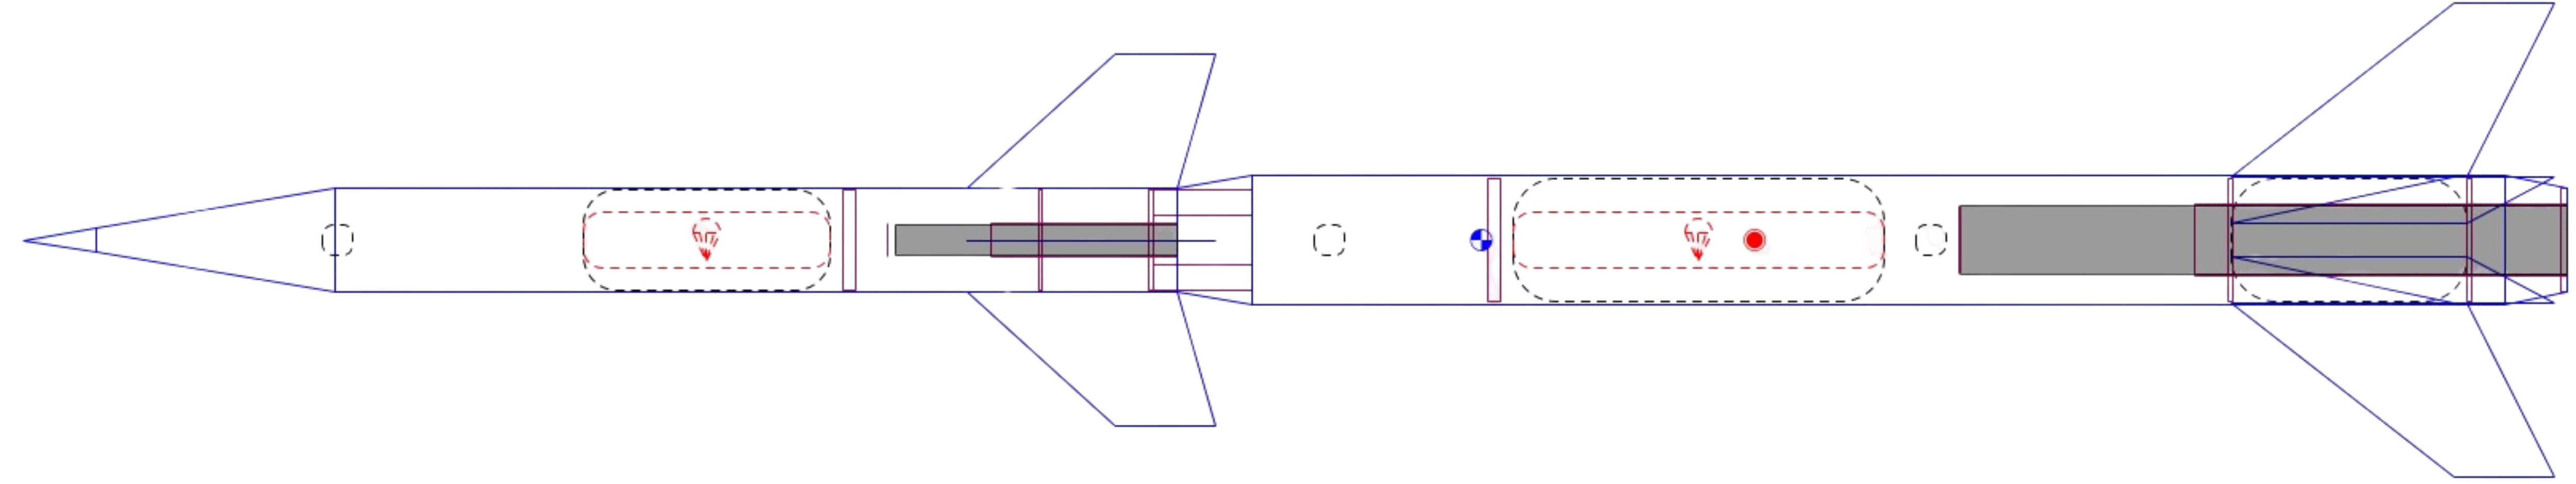
\includegraphics[width=\textwidth]{figures/sp02_ork.png}
    \caption{Modélisation de la fusée SP-02 dans \gls{OpenRocket}}
    \label{fig:sp02_ork_model}
\end{figure}

\vfill

\newpage

\subsubsection{Résultats}
\label{subsubsec:stabilite_resultats}


\subsubsubsection{Configuration adoptée}
Après plusieurs itérations de conception et d'analyses, nous avons abouti à une configuration générale composée d'un jeux de 4 ailerons de
type trapezoïdal sur chaques étages, une coiffe conique, un changement de diamètre entre les deux étages et un rétreint au niveau du bas du
premier étage.\\

Bien que le nombre d'ailerons soit le même pour les deux étages, entrainant le questionnement de l'effet de masquage des surfaces portantes
du premier étage par le second, le choix a été fait de non pas aligner ces deux jeux d'ailerons mais de les décaler de 15° l'un par rapport
à l'autre. Ceci répond directemnt à la règle STAB6 du \acrshort{CDC} et à sa partie "contrôle" :

\begin{quote}
    (Règle) \textit{"STAB6 : Dans le cas d’une fusée à deux jeux d’ailerons dont les ailerons sont alignés, la fusée doit être stable à la
    fois sans tenir compte des effets de masquage du jeu d’aileron inférieur par le jeu d’aileron supérieur et à la fois en tenant compte de
    cette interaction.}\newline\cite[p.~34]{CDC_BiEtage}
\end{quote}

\begin{quote}
    (Contrôle) \textit{"STAB6 : On considère que deux jeux d’ailerons sont alignés s’il est possible, vue du vent relatif, de trouver deux
    ailerons consécutifs séparés par un angle de 10° ou moins.}\newline\cite[p.~34]{CDC_BiEtage}
\end{quote}

Le choix de ces 15° de décalage permet donc de s'affranchir de cette règle et de simplifier les analyses de stabilité. Cela entraine
néanmoins une légère diminution de la place disponible entre les ailerons de la fusée et la rampe de lancement car nous passons d'un angle
de 90° entre deux ailerons consécutifs à un angle de 75°. Cette diminution a été jugée acceptable au regard des bénéfices apportés par ce
décalage.\\

\subsubsubsection{Résultats des analyses}

De cette étude de stabilité, trois graphiques principaux ont été extraits, présentés dans la figure \ref{fig:stabilite_resultats}.
Ces graphiques montrent l'évolution des marges de stabilité longitudinale de la fusée SP-02 complète, du premier étage et du second étage en
fonction de la variation de masse de propergol consommée durant le vol.\\

\begin{figure}[h!]
    \centering
    \begin{subfigure}{0.32\textwidth}
        \centering
        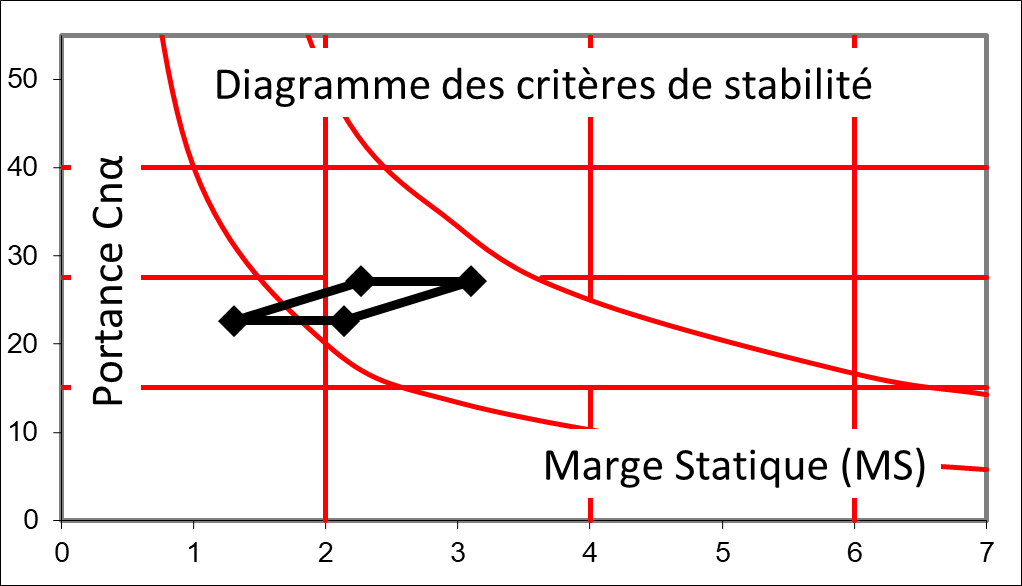
\includegraphics[width=\textwidth]{figures/stabtraj_ensemble.png}
        \caption{Fusée SP-02 complète}
        \label{fig:stabilite_sp02}
    \end{subfigure}
    \begin{subfigure}{0.32\textwidth}
        \centering
        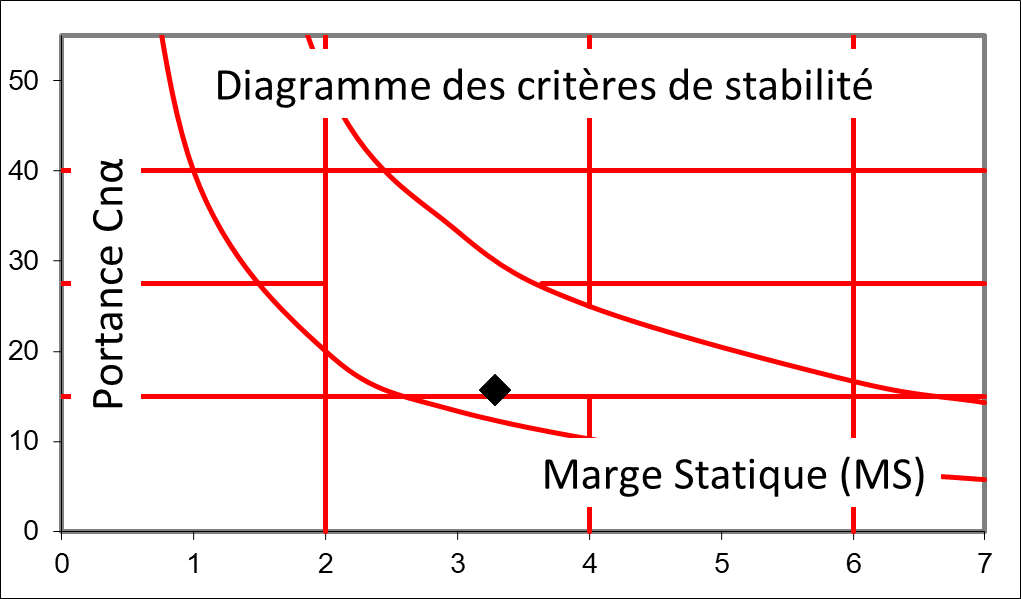
\includegraphics[width=\textwidth]{figures/stabtraj_alpha.png}
        \caption{Premier étage}
        \label{fig:stabilite_etage1}
    \end{subfigure}
    \begin{subfigure}{0.32\textwidth}
        \centering
        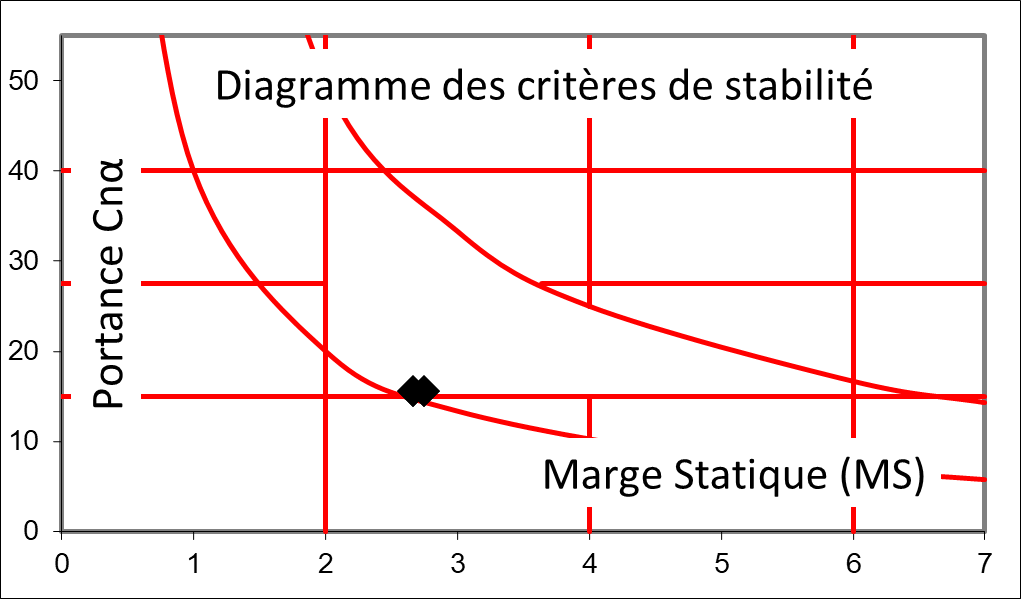
\includegraphics[width=\textwidth]{figures/stabtraj_beta.png}
        \caption{Second étage}
        \label{fig:stabilite_etage2}
    \end{subfigure}
    \caption{Résultats des analyses de stabilité longitudinale de la fusée SP-02 et de ses étages (\gls{Stabtraj})}
    \label{fig:stabilite_resultats}
\end{figure}

Nous observons que le graphique de la figure \ref{fig:stabilite_sp02} montre que les marges de stabilitées de la fusée au complet forment un
prisme dû à l'effet de masquage. Ainsi, bien qu'une partie du prisme soit en dehors de la zone de stabilité (marge de statique $< 2$), seule
la droite supérieure du prime à portance constante est celle qui compte effectivement. Cette droite étant inclus dans la zone de stabilité, la
fusée SP-02 est donc stable durant toute la phase propulsée de son vol.\\

On remarque également que les marges de stabilité des deux étages individuellement, sont eux aussi stables bien que collé à la limite
inférieur de portance. Après discussion avec notre encadrant technique de la \acrshort{RCE}-1, il a été conclue que cette situation était
acceptable étant donné qu'au moment de la séparation des étages, ces deux étages auront déjà des vitesses relativement élevées, assurant une
stabilité dynamique suffisante malgré une portance faible.\\

Ces résultats ont été corrélés avec ceux obtenus via \gls{OpenRocket}, qui confirment la stabilité de la fusée SP-02.

\newpage
